\section{Referencia de la Clase Busqueda\-Provincia}
\label{classBusquedaProvincia}\index{BusquedaProvincia@{BusquedaProvincia}}
Permite buscar y seleccionar una provincia.  


{\tt \#include $<$busquedaprovincia.h$>$}

Diagrama de colaboraci\'{o}n para Busqueda\-Provincia:\begin{figure}[H]
\begin{center}
\leavevmode
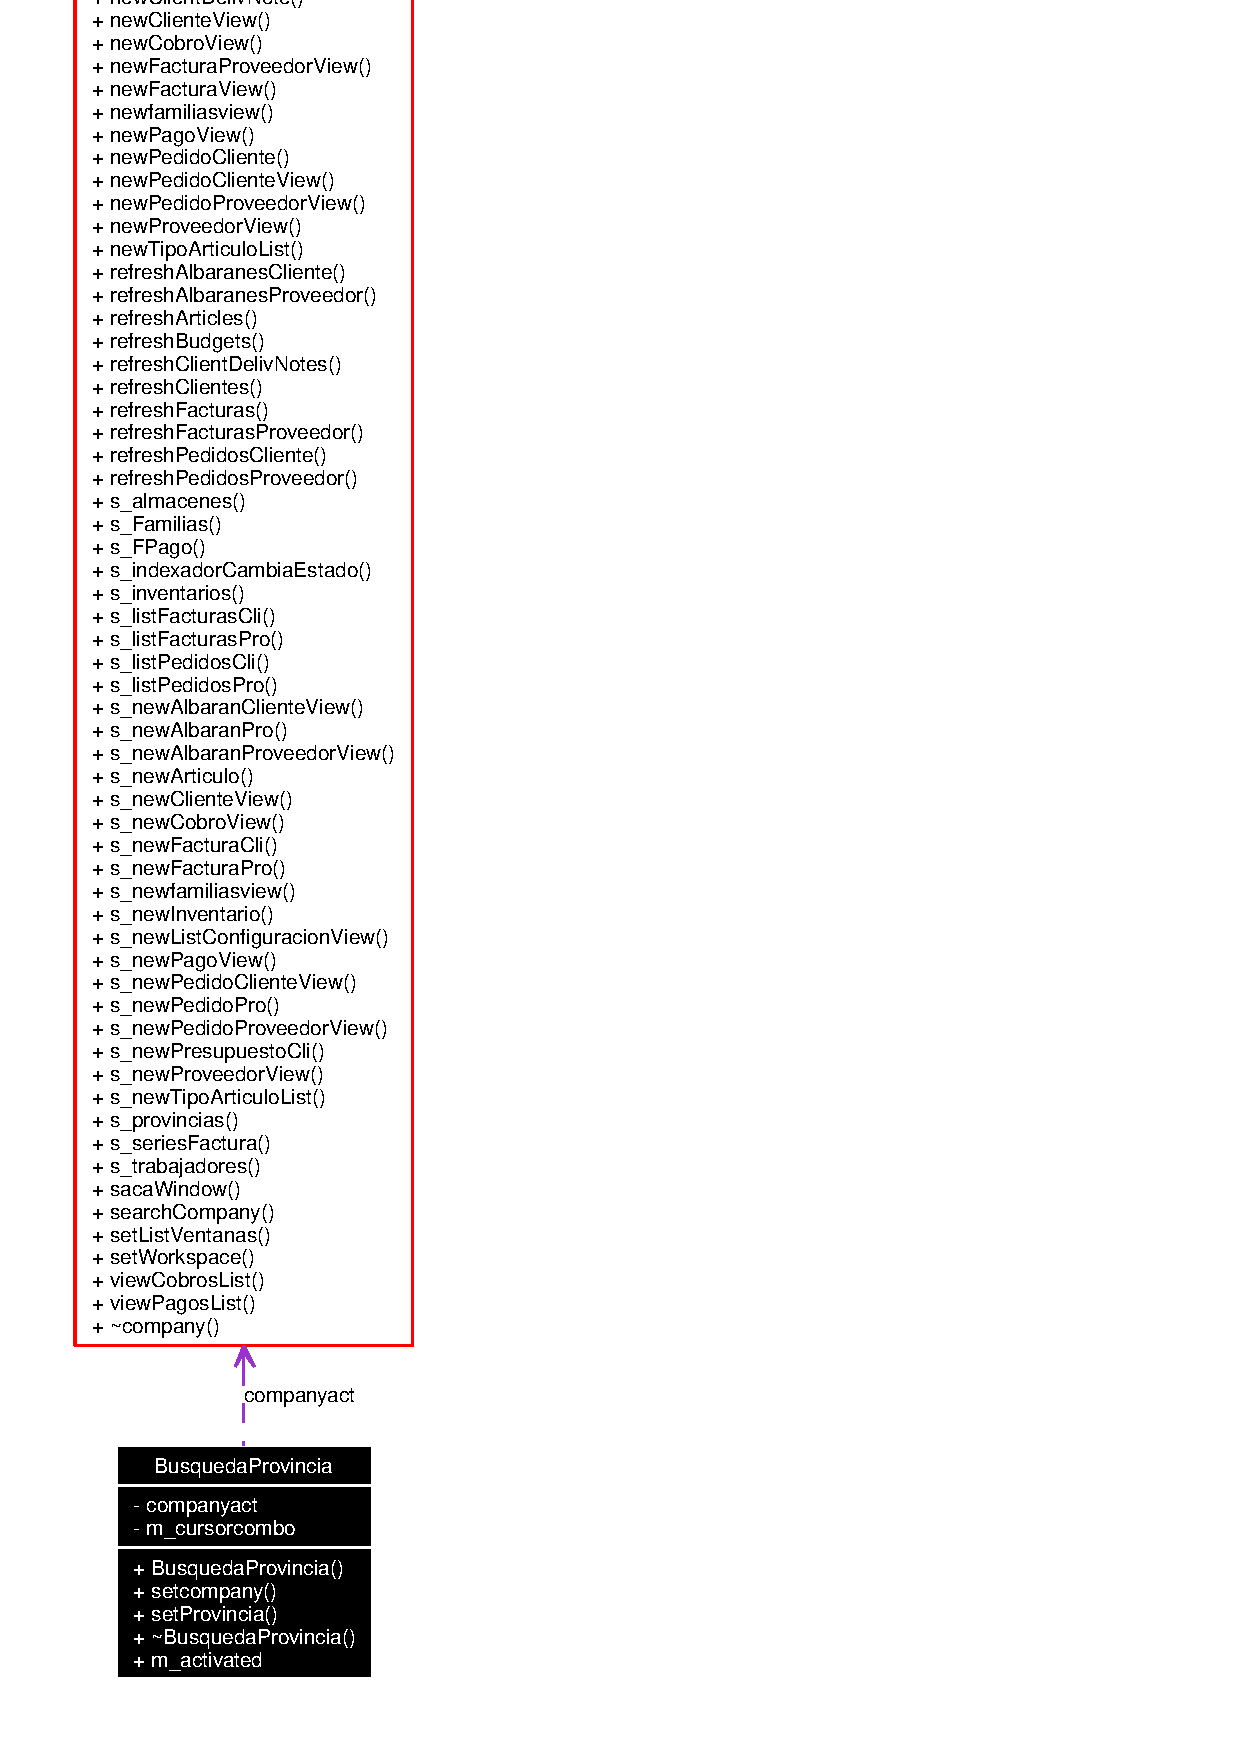
\includegraphics[width=99pt]{classBusquedaProvincia__coll__graph}
\end{center}
\end{figure}
\subsection*{Slots p\'{u}blicos}
\begin{CompactItemize}
\item 
void {\bf m\_\-activated} (int index)\label{classBusquedaProvincia_i0}

\end{CompactItemize}
\subsection*{Se\~{n}ales}
\begin{CompactItemize}
\item 
void {\bf value\-Changed} (QString)\label{classBusquedaProvincia_l0}

\end{CompactItemize}
\subsection*{M\'{e}todos p\'{u}blicos}
\begin{CompactItemize}
\item 
{\bf Busqueda\-Provincia} (QWidget $\ast$parent=0)\label{classBusquedaProvincia_a0}

\item 
void {\bf setcompany} ({\bf company} $\ast$comp)\label{classBusquedaProvincia_a1}

\item 
virtual void {\bf set\-Provincia} (QString provincia)\label{classBusquedaProvincia_a2}

\end{CompactItemize}


\subsection{Descripci\'{o}n detallada}
Permite buscar y seleccionar una provincia. 

Muestra la parte del formulario que permite buscar y seleccionar una provincia. 



La documentaci\'{o}n para esta clase fu\'{e} generada a partir de los siguientes archivos:\begin{CompactItemize}
\item 
busquedaprovincia.h\item 
busquedaprovincia.cpp\end{CompactItemize}
